\section{Resultados}
\subsection{Comparação de eficiencia}
Cada kernel foi executado 3000 vezes em sequência. A GPU tem um mecânismo que faz um cache do código do kernel e também
da memória que ele utiliza, então podemos desconsiderar a comunicação da CPU com a GPU neste caso, deixando os nossos resultados 
mais próximos do tempo de execução dos kernels.

É importante levar em conta que a GPU não estava rodando somente o kernel, já que os drivers necessários para a execução 
do mesmo estão atrelados ao X Window System, então o kernel sofreu interrupções na GPU, para que a interface gráfica do 
Ubuntu fosse renderizada.

\subsubsection{Kernel memory-bound}
Os resultados dos kernels memory-bound:

\begin{figure}[H]
  \begin{center}
    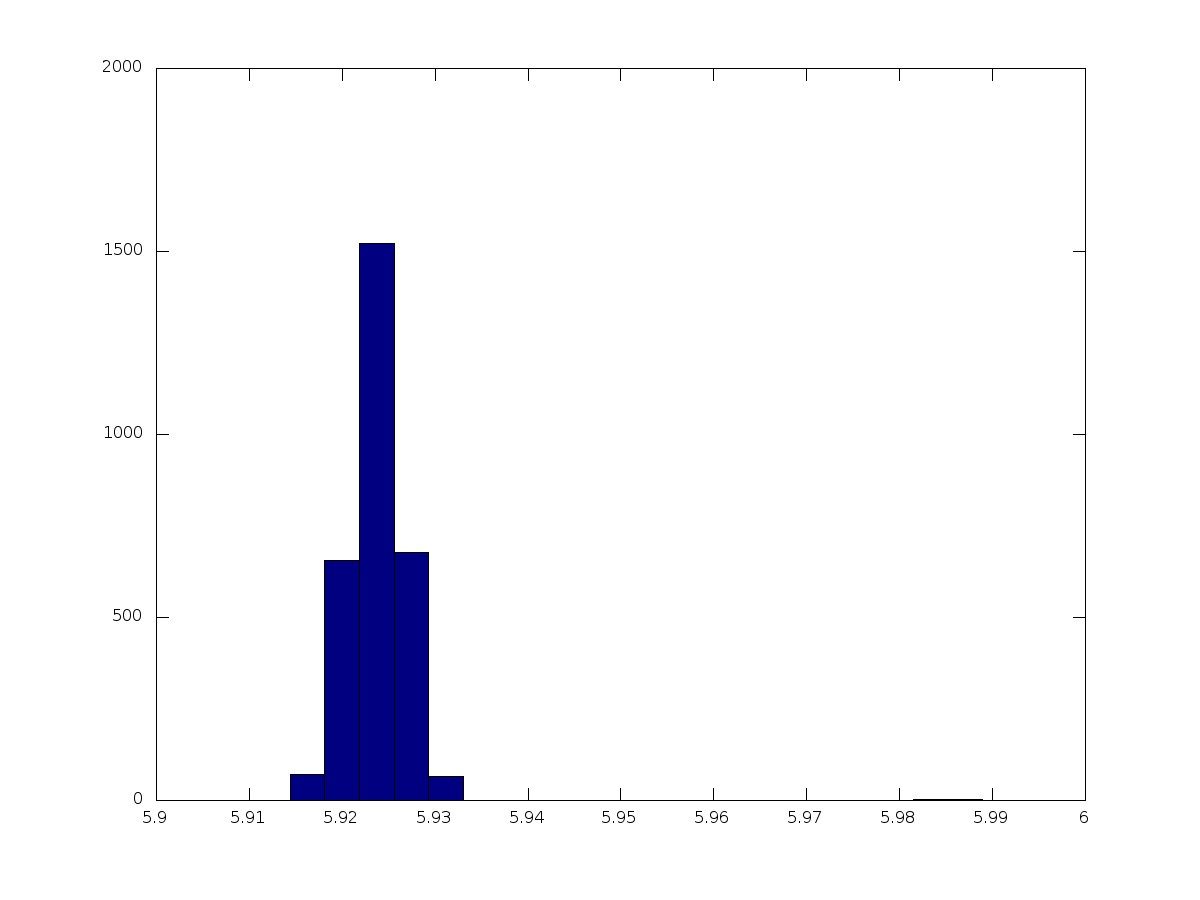
\includegraphics[scale=0.3]{resultados_cuda_memory_histo.jpg}
    \label{fig:Kernel Memory-Bound CUDA}
    \caption{Kernel Memory-Bound CUDA}
  \end{center}
\end{figure}

\begin{figure}[H]
  \begin{center}
    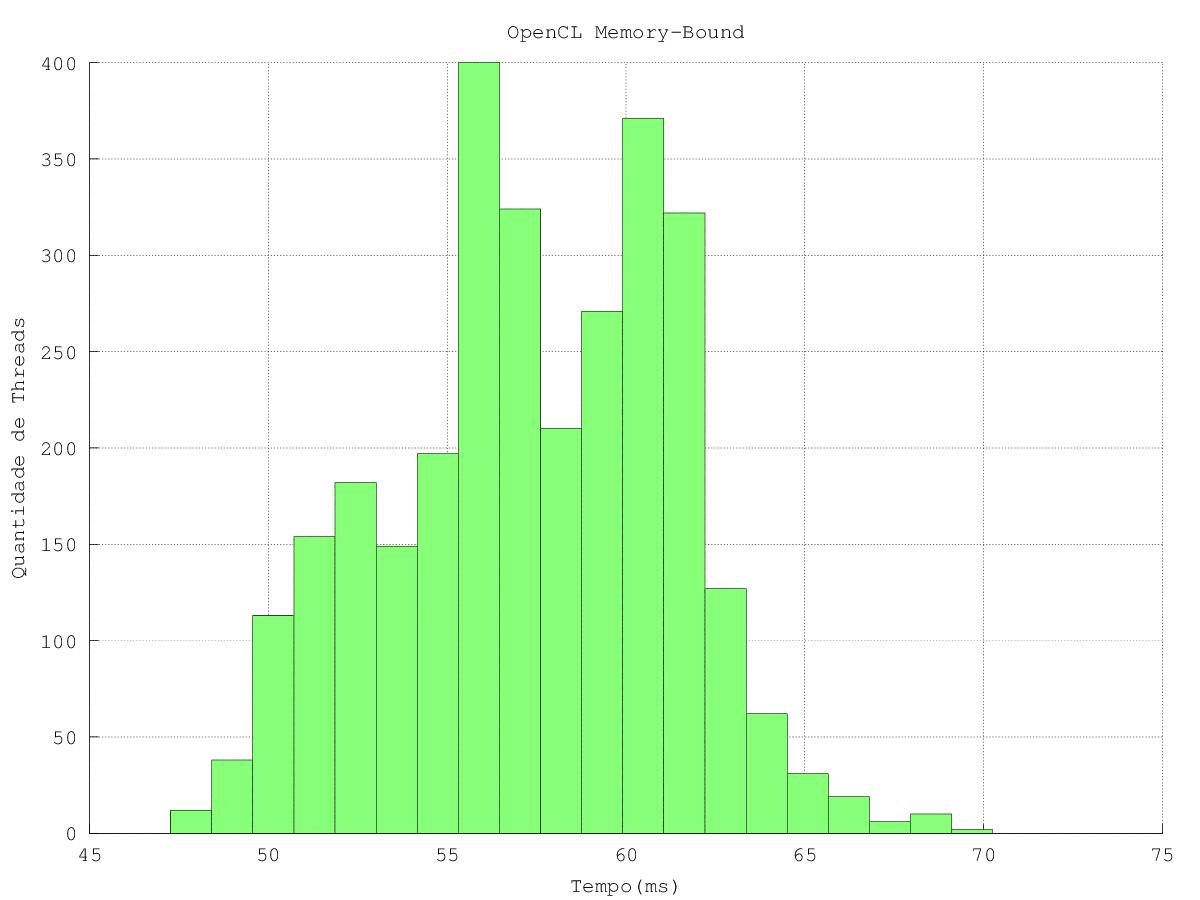
\includegraphics[scale=0.3]{resultados_opencl_memory_histo.jpg}
    \label{fig:Kernel Memory-Bound OpenCL}
    \caption{Kernel Memory-Bound OpenCL}
  \end{center}
\end{figure}

\subsubsection{Kernel processing-bound}
\subsection{Comparação dos .ptx}
